\documentclass[bachelor, och, labwork]{shiza}
% параметр - тип обучения - одно из значений:
%    spec     - специальность
%    bachelor - бакалавриат (по умолчанию)
%    master   - магистратура
% параметр - форма обучения - одно из значений:
%    och   - очное (по умолчанию)
%    zaoch - заочное
% параметр - тип работы - одно из значений:
%    referat    - реферат
%    coursework - курсовая работа (по умолчанию)
%    diploma    - дипломная работа
%    pract      - отчет по практике
% параметр - включение шрифта
%    times    - включение шрифта Times New Roman (если установлен)
%               по умолчанию выключен
\usepackage{subfigure}
\usepackage{tikz,pgfplots}
\pgfplotsset{compat=1.5}
\usepackage{float}

%\usepackage{titlesec}
\setcounter{secnumdepth}{4}
%\titleformat{\paragraph}
%{\normalfont\normalsize}{\theparagraph}{1em}{}
%\titlespacing*{\paragraph}
%{35.5pt}{3.25ex plus 1ex minus .2ex}{1.5ex plus .2ex}

\titleformat{\paragraph}[block]
{\hspace{1.25cm}\normalfont}
{\theparagraph}{1ex}{}
\titlespacing{\paragraph}
{0cm}{2ex plus 1ex minus .2ex}{.4ex plus.2ex}

% --------------------------------------------------------------------------%


\usepackage[T2A]{fontenc}
\usepackage[utf8]{inputenc}
\usepackage{graphicx}
\graphicspath{ {./images/} }
\usepackage{tempora}

\usepackage[sort,compress]{cite}
\usepackage{amsmath}
\usepackage{amssymb}
\usepackage{amsthm}
\usepackage{fancyvrb}
\usepackage{listings}
\usepackage{listingsutf8}
\usepackage{longtable}
\usepackage{array}
\usepackage[english,russian]{babel}

% \usepackage[colorlinks=true]{hyperref}
\usepackage{url}

\usepackage{underscore}
\usepackage{setspace}
\usepackage{indentfirst} 
\usepackage{mathtools}
\usepackage{amsfonts}
\usepackage{enumitem}
\usepackage{tikz}

\newcommand{\eqdef}{\stackrel {\rm def}{=}}
\newcommand{\specialcell}[2][c]{%
\begin{tabular}[#1]{@{}c@{}}#2\end{tabular}}

\renewcommand\theFancyVerbLine{\small\arabic{FancyVerbLine}}

\newtheorem{lem}{Лемма}

\begin{document}

% Кафедра (в родительном падеже)
\chair{}

% Тема работы
\title{Настройка ЛВС}

% Курс
\course{2}

% Группа
\group{231}

% Факультет (в родительном падеже) (по умолчанию "факультета КНиИТ")
\department{факультета КНиИТ}

% Специальность/направление код - наименование
%\napravlenie{09.03.04 "--- Программная инженерия}
%\napravlenie{010500 "--- Математическое обеспечение и администрирование информационных систем}
%\napravlenie{230100 "--- Информатика и вычислительная техника}
%\napravlenie{231000 "--- Программная инженерия}
\napravlenie{100501 "--- Компьютерная безопасность}

% Для студентки. Для работы студента следующая команда не нужна.
% \studenttitle{Студентки}

% Фамилия, имя, отчество в родительном падеже
\author{Окунькова Сергея Викторовича}

% Заведующий кафедрой
% \chtitle{} % степень, звание
% \chname{}

%Научный руководитель (для реферата преподаватель проверяющий работу)
\satitle{ассистент} %должность, степень, звание
\saname{А. А. Фомин}

% Руководитель практики от организации (только для практики,
% для остальных типов работ не используется)
% \patitle{к.ф.-м.н.}
% \paname{С.~В.~Миронов}

% Семестр (только для практики, для остальных
% типов работ не используется)
%\term{8}

% Наименование практики (только для практики, для остальных
% типов работ не используется)
%\practtype{преддипломная}

% Продолжительность практики (количество недель) (только для практики,
% для остальных типов работ не используется)
%\duration{4}

% Даты начала и окончания практики (только для практики, для остальных
% типов работ не используется)
%\practStart{30.04.2019}
%\practFinish{27.05.2019}

% Год выполнения отчета
\date{2021}

\maketitle

% Включение нумерации рисунков, формул и таблиц по разделам
% (по умолчанию - нумерация сквозная)
% (допускается оба вида нумерации)
% \secNumbering

%-------------------------------------------------------------------------------------------


\begin{enumerate}
    
    \item Составить и заполнить адресную таблицу.
    
    \begin{figure}[H]
        \centering      %размер рисунка       здесь находится название файла рисунка, без указания формата
        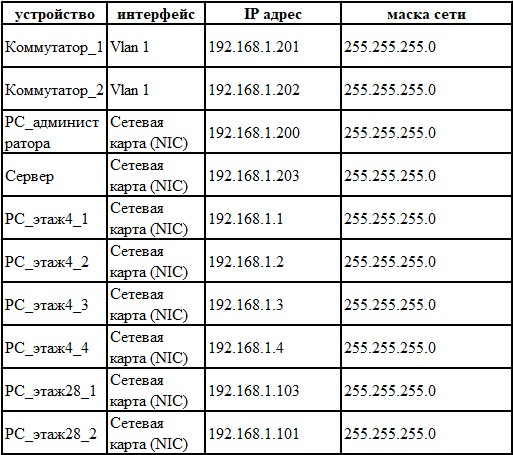
\includegraphics[width=1\textwidth]{1}
        \caption{Таблица IP адрессов устройств в заданной конфигурации}
        \label{fig:image1}
    \end{figure}

    \item Запустите Packet Tracer и воспроизведите физическую конфигурацию.
    
    \begin{figure}[H]
        \centering      %размер рисунка       здесь находится название файла рисунка, без указания формата
        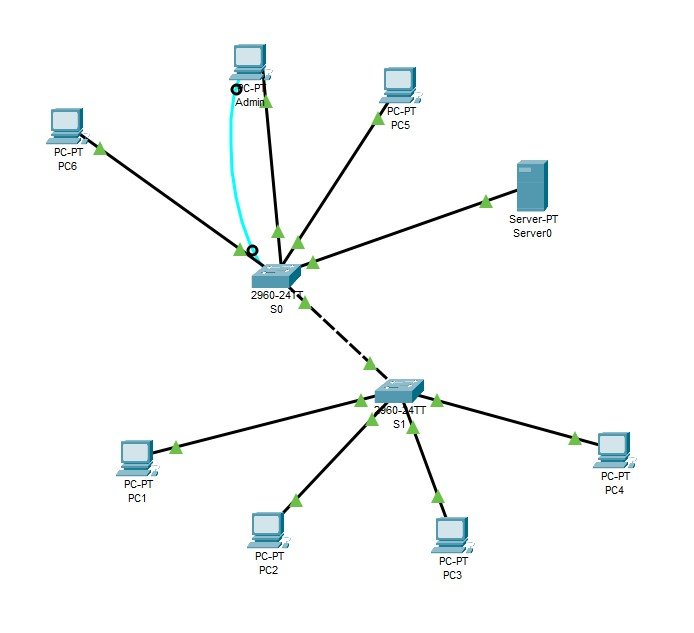
\includegraphics[width=1\textwidth]{2}
        \caption{Заданная конфигурация}
        \label{fig:image1}
    \end{figure}

    \item С помощью компьютера администратора и консольного подключения выполните базовое конфигурирование коммутаторов. Для каждого из них:
    
    - задайте уникальное имя
    
    - задайте пароль на консольное подключение
    
    - задайте пароль на доступ к привилегированному пользовательскому режиму
    
    - установите уведомление MOTD, сообщающее о недопустимости несанкционированного доступа к коммутатору
    
    - сохраните конфигурацию, чтобы она продолжала использоваться после перезагрузки устройства
    
    - назначьте IP адрес интерфейсу vlan 1
    
    - включите этот интерфейс
    
    - сохраните конфигурацию
    
    - еще раз внимательно просмотрите конфигурацию и убедитесь что все линии виртуальных терминалов (vty) коммутаторов готовы для приема удаленных подключений и не защищены паролями
    
    -при необходимости внесите исправления в конфигурацию и сохраните её
    
    - отключите консольный кабель

    Разберем все эти действия на примере коммутатора на 28-м этаже:

    \begin{figure}[H]
        \centering      %размер рисунка       здесь находится название файла рисунка, без указания формата
        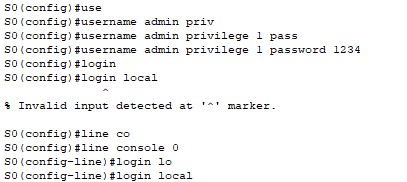
\includegraphics[width=0.7\textwidth]{3}
        \caption{Задание пароль на консольное подключение}
        \label{fig:image1}
    \end{figure}
    
    \begin{figure}[H]
        \centering      %размер рисунка       здесь находится название файла рисунка, без указания формата
        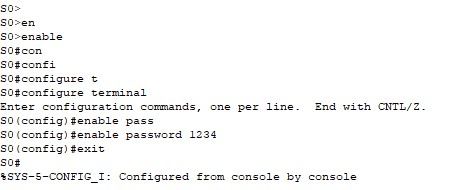
\includegraphics[width=0.7\textwidth]{4}
        \caption{Задание пароль на доступ к привилегированному пользовательскому режиму}
        \label{fig:image1}
    \end{figure}

    \begin{figure}[H]
        \centering      %размер рисунка       здесь находится название файла рисунка, без указания формата
        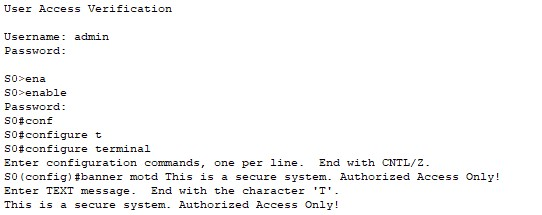
\includegraphics[width=0.7\textwidth]{5}
        \caption{Установка уведомление MOTD, сообщающего о недопустимости несанкционированного доступа к коммутатору}
        \label{fig:image1}
    \end{figure}

    \begin{figure}[H]
        \centering      %размер рисунка       здесь находится название файла рисунка, без указания формата
        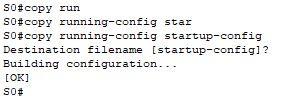
\includegraphics[width=0.7\textwidth]{6}
        \caption{Сохранение конфигурации}
        \label{fig:image1}
    \end{figure}

    \begin{figure}[H]
        \centering      %размер рисунка       здесь находится название файла рисунка, без указания формата
        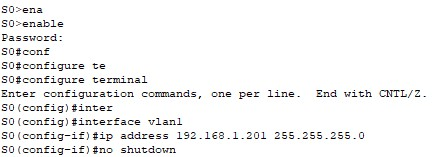
\includegraphics[width=0.7\textwidth]{7}
        \caption{Назначение IP адрес интерфейсу vlan 1}
        \label{fig:image1}
    \end{figure}

    \begin{figure}[H]
        \centering      %размер рисунка       здесь находится название файла рисунка, без указания формата
        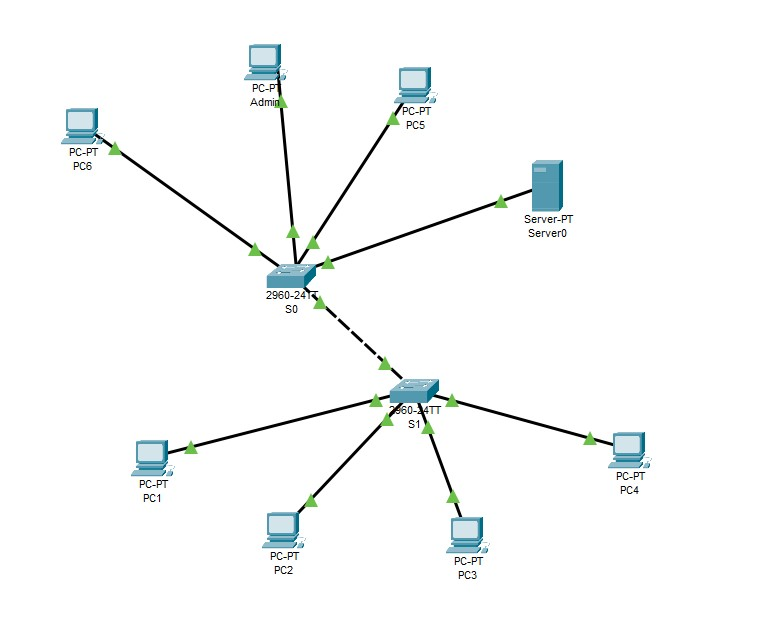
\includegraphics[width=1\textwidth]{8}
        \caption{Отключение консольного кабеля}
        \label{fig:image1}
    \end{figure}

    \item Выполните конфигурирование IP настроек на всех рабочих станциях, сервере и компьютере администратора.
    
    \begin{figure}[H]
        \centering      %размер рисунка       здесь находится название файла рисунка, без указания формата
        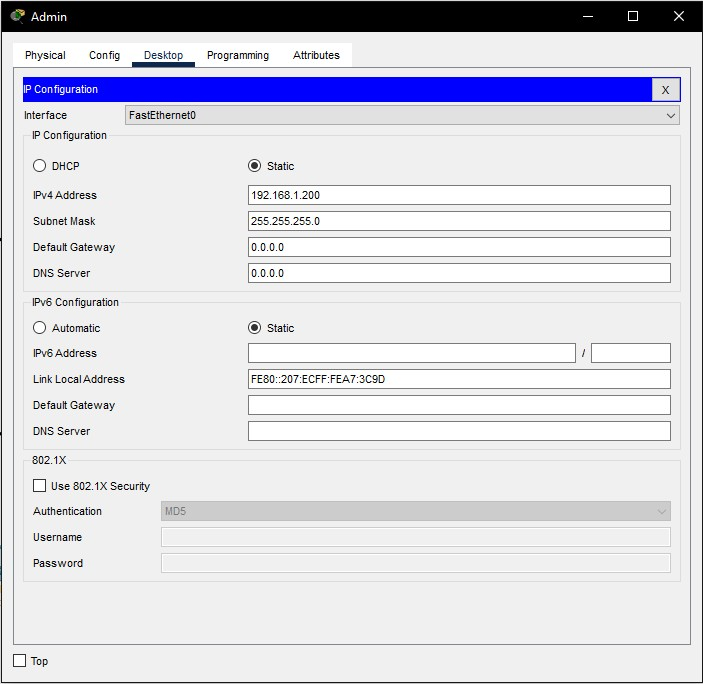
\includegraphics[width=1\textwidth]{9}
        \caption{Конфигурирование IP настроек на компьютере администратора}
        \label{fig:image1}
    \end{figure}

    Остальные настройки выполним по аналогии

    \item Проверьте доступность с компьютера администратора всех рабочих станций и сервера.
    
    \begin{figure}[H]
        \centering      %размер рисунка       здесь находится название файла рисунка, без указания формата
        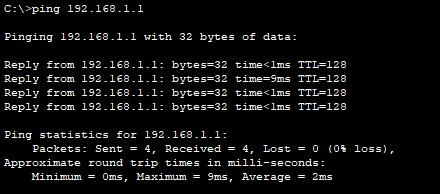
\includegraphics[width=1\textwidth]{10}
        \caption{Проверка доступности PC1 на 4-м этаже командой ping}
        \label{fig:image1}
    \end{figure}

    Проверив доступность остальных элементов конфигурации по аналогии, вышло, что они все доступны.

    \item Проверьте доступность с компьютера администратора первого и второго коммутаторов.

    \begin{figure}[H]
        \centering      %размер рисунка       здесь находится название файла рисунка, без указания формата
        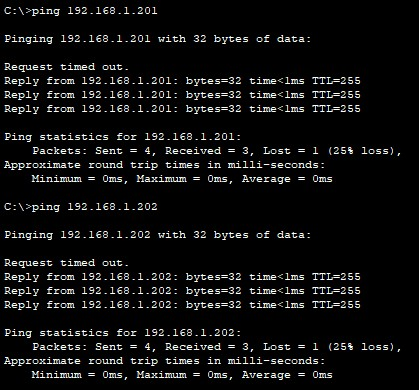
\includegraphics[width=0.75\textwidth]{11}
        \caption{Проверка доступности коммутаторов командой ping}
        \label{fig:image1}
    \end{figure}

    \item Используя протокол Telnet, выполните удалённое подключение к каждому из коммутаторов
    
    \begin{figure}[H]
        \centering      %размер рисунка       здесь находится название файла рисунка, без указания формата
        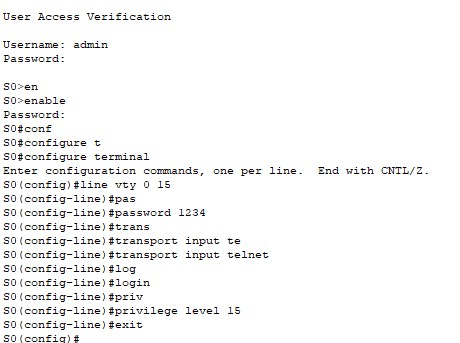
\includegraphics[width=0.75\textwidth]{12}
        \caption{Настройка протокола Telnet}
        \label{fig:image1}
    \end{figure}

    \begin{figure}[H]
        \centering      %размер рисунка       здесь находится название файла рисунка, без указания формата
        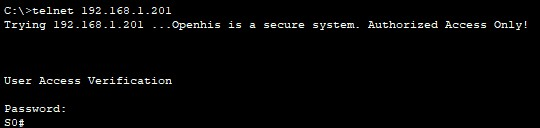
\includegraphics[width=0.7\textwidth]{13}
        \caption{Удаленное подключение к S0 с помощью протокола Telnet}
        \label{fig:image1}
    \end{figure}

    \item Проверьте сетевую доступность для каждого коммутатора другого коммутатора и компьютера администратора.
    
    \begin{figure}[H]
        \centering      %размер рисунка       здесь находится название файла рисунка, без указания формата
        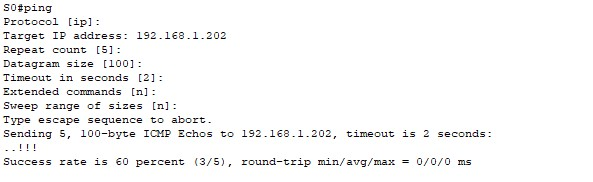
\includegraphics[width=0.7\textwidth]{14}
        \caption{Проверка сетевой доступности коммутаторов}
        \label{fig:image1}
    \end{figure}

    \begin{figure}[H]
        \centering      %размер рисунка       здесь находится название файла рисунка, без указания формата
        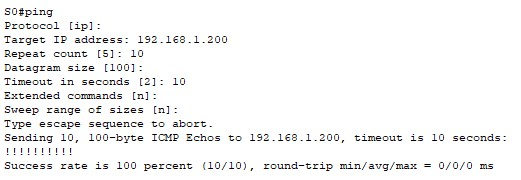
\includegraphics[width=0.7\textwidth]{15}
        \caption{Проверка сетевой доступности коммутатора и пк админа}
        \label{fig:image1}
    \end{figure}

    \item Установите пароли доступа на линии виртуальных терминалов и проверьте их действие
    
    При настройке протокола telnet я уже поставил пароль, что можно увидеть на рисунке 12 

\end{enumerate}

\end{document}
